\section{Preliminary}
In this section, we introduce some preliminary knowledge. First, the basis of LSTM, GAN and DCGAN is presented.  We then introduce the preliminary knowledge of ICPs and their common features. Lastly, we give an overview of fuzz testing and its application in finding ICPs' vulnerabilities.

\subsection{Long Short-Term memory}
Hochreiter and Schmidhuber (1997) first proposed LSTM to overcome the gradient vanishing problem of RNN (Recurrent Neural Networks). It is a special RNN that introduces an adaptive gating mechanism which can decides the degree to keep the previous state and avoid the problem of long-tern dependencies. Given a sequence $S = {x1, x2, …, xl}$, where $l$ is the length of input text, LSTM processes it word by word. At time-step $t$, the memory $c_{t}$ and the hidden state $h_{t}$ are updated with the following equations:
\begin{equation}
\left[ \begin{array}{c}
\Gamma _u^{ < t > }\\
\Gamma _f^{ < t > }\\
\Gamma _o^{ < t > }\\
{{\hat c}_t}
\end{array} \right] = \left[ \begin{array}{c}
\sigma \\
\sigma \\
\sigma \\
\tanh 
\end{array} \right]W \cdot \left[ {{h_{t - 1}},{x_t}} \right]
\end{equation}
\begin{equation}
{c_t} = \Gamma _f^{ < t > } \odot {c_{t - 1}} + \Gamma _u^{ < t > } \odot {\hat c_t}
\end{equation}
\begin{equation}
{h_t} = \Gamma _o^{ < t > } \odot \tanh ({c_t})
\end{equation}
where $x_{t}$ is the input at the current time-step, $\Gamma _u$, $\Gamma _f$ and $\Gamma _o$ is the update gate activation, forget gate activation and output gate activation respectively, $\hat{c}$ is the current cell state, $\sigma$ denotes the logistic sigmoid function and $\odot$ denotes element-wise multiplication.

\subsection{Generative Adversarial Networks}
Generative Adversarial Networks, proposed by Goodfellow and others, is a promising framework to guide the training of generative models. Specifically, in GAN, a discriminative network $D$ (discriminator) learns to distinguish whether a given data instance is real or not, and a generative network $G$ (generator) learns to confuse discriminator by generating fake but plausible data. 

In this adversarial network framework, the goal of the training generation model is to obtain a probability distribution of $P_z$, which approximates the distribution $P_x$ of the real data $x$. In order to achieve this goal, a known distribution (such as Gaussian distribution, uniform distribution) is used to sample and get the ``noise data " (represented by $z$) in the first place. Then, these ``noise data" are input into the generation model, and the training of the generation model is carried out. After the training of the generator is finished, simulated data is output. 

In this study, we utilize this feature to generate simulated sequence messages. Notably, when applying deep adversarial learning to fuzz testing ICPs, we expect the generated data to have a correct message format but with various message content so that the code coverage and testing depth can be guaranteed. 

%\begin{figure}[htbp]
%\centering
%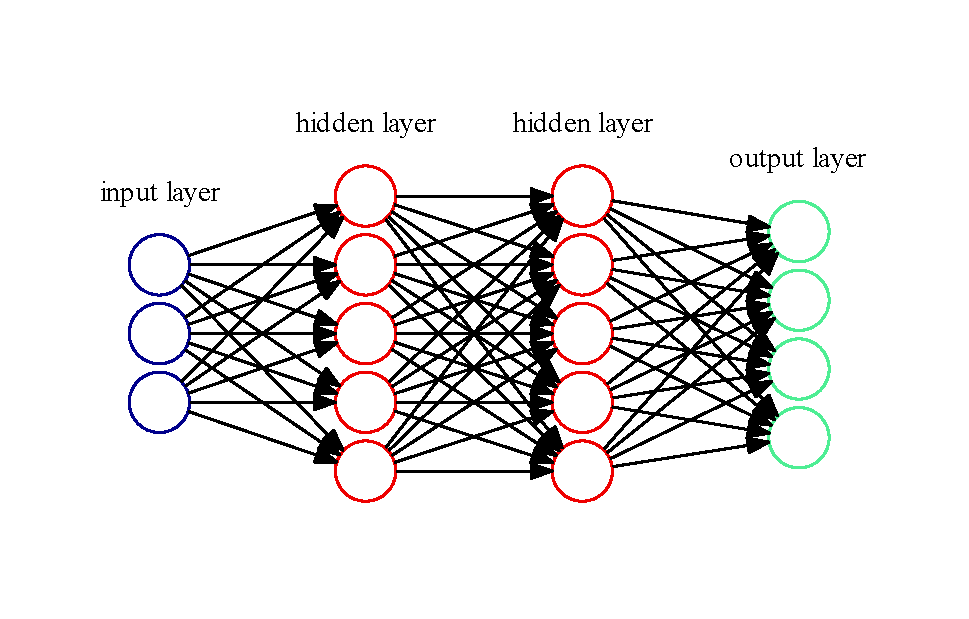
\includegraphics[scale=0.4]{FIGURE/FIGURE_NNSTRUCT.pdf}
%\caption{Multilayer Perceptron}
%\label{FIGURE_NNSTRUCT}
%\end{figure}

\subsection{Deep Convolution Generative Adversarial Networks}
Prior to introducing DCGAN, it is necessary to briefly introduce CNNs (Convolution Neural Networks), which have recently enjoyed great success in image and video recognition. Its success is mainly due to the large public image repositories, such as ImageNet, and high-performance computing systems, such as GPUs (Graphics Processing Units) or large-scale distributed clusters. Because the pooling layer has no weights, no parameters and only a few hyperparameters, one convention comprises one convolutional layer part and one pooling layer part in general. A typical CNN consists of many layers, including the input layer, conventions, the fully-connected layer, the output layer, etc.

Recently, NLP communities pay more and more attention to CNN and have achieved favorable results in various text classification tasks \cite{kim2014convolutional,zhang2015character}. Different from RNNs accomplished in time-related problems, CNN is good at learning spatial structure features. Actually, most ICPs’ messages have the following features: concise format, limited length and compact structure. This makes CNN a better way to solve this kind of problem \cite{kim2014convolutional}. After proper preprocessing via Bi-LSTM which adds the location feature in the input, each filter in CNN can be regarded as a detector that detects whether a functional unit in the data frame is correct \cite{adel2016exploring}, which is conducive to grasping the format features of the sequence data in ICS.  Hence in this study, CNN serves as the generator and the discriminator in DCGAN accordingly.

DCGAN is proposed by Alec Radford et al. \cite{radford2015unsupervised} to bridge the gap between the success of CNNs for supervised learning and unsupervised learning. They extend GAN to the CNN domain and invent a structure called deep convolution generative adversarial networks (DCGAN) that have certain architectural constraints. This innovation combines the advantages of CNN in processing multidimensional features and the idea of deep adversarial learning. Due to the constraints, DCGAN largely overcomes the problem of unstable training of GANs, such as non-convergence, vanishing gradient and mode collapse.  These constraints are listed in Table \uppercase\expandafter{\romannumeral1}. We designed our model architecture based on the constraints.


\begin{table}[htbp]
\caption{Architecture guidelines for stable Deep Convolutional Generative Adversarial Networks}
\label{table_example}
\centering
\begin{tabular}{|c|c|}
\hline
\bfseries \# & \bfseries Architecture constraints\\
\hline
1 & \multicolumn{1}{m{7cm}|}{Replace any pooling layers with strided convolutions (discriminator) and fractional-strided convolutions (generator).}\\
\hline
2 & \multicolumn{1}{m{7cm}|}{Use batch normal in both the generator and the discriminator.} \\
\hline
3 & \multicolumn{1}{m{7cm}|}{Remove fully connected hidden layers for deeper architectures.} \\
\hline
4 & \multicolumn{1}{m{7cm}|}{Use ReLU activation in the generator for all layers except for the output, which uses Tanh.}\\
\hline
5 & \multicolumn{1}{m{7cm}|}{Use LeakyReLU activation in the discriminator for all layers.}\\
\hline
\end{tabular}
\end{table}


\subsection{Industrial Control Protocols}
ICPs refers to the communication protocol deployed in ICSs. As a class of systems, ICS has its characteristics, such as requiring high real-time performance and just providing several specific functions. Correspondingly, ICP's message format tends to be concise. ICS consist of master stations and slave stations. The data transmission and operation control between them are realized through the ICP in it. Currently, various ICPs operate in a wide variety of ICSs around the world. Therefore, it is important to maintain ICPs' safety and security. Except for the popular ICPs, Some ICPs are modified from the existing protocols or solely designed. These ICPs may have no clear specifications. Thus, the manual-based fuzz testing method will suffer from this.

\subsection{Fuzz Testing}
Fuzz testing is a quick and cost-effective method for finding severe security defects in software. Traditionally, fuzz testing tools apply random mutations to well-formed inputs of a program and test the resulting values. Besides, fuzzing is a brute force vulnerability method, in which it uses a large amount of malicious input to have stress tests on the target. As industrial control networks become more and more interconnected, flaws in the implementations of ICP could allow a malicious party to attack vulnerable systems remotely over the internet. To avoid this, we use fuzzing to discover the flaws in advance. The workflow is shown in Fig.  \ref{FigFuzzingFlow}.
\begin{figure}[htbp]
	\centering
	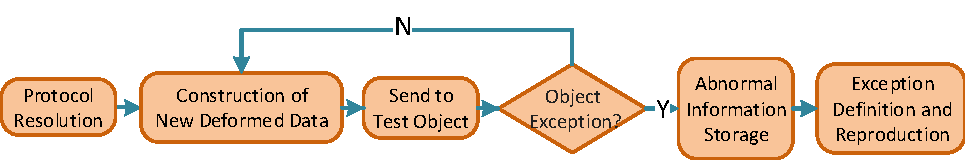
\includegraphics[width=3.5in]{FIGURE_LV/FigFuzzingFlow.pdf}
	\caption{General workflow of fuzzing test}
	\label{FigFuzzingFlow}
\end{figure}

